Wir möchten euch außerdem noch ein paar Infos zu den Veranstaltungen geben, die euch im ersten Semester erwarten, damit ihr nichts wichtiges verpasst.

\subsubsection*{Informatik 1}
Informatik 1 ist die Grundlagenvorlesung der Informatik, in der ihr lernt zu programmieren. Hierfür sind keine Vorkenntnisse nötig. In der zweimal die Woche stattfindenden Vorlesung stellt euch der Professor immer neue Konzepte vor, welche ihr dann in den Übungen zuhause und im Tutorium üben könnt und solltet. Man hat meist eine Woche Zeit, die Aufgaben zu bearbeiten und abzugeben. Ein Tutor korrigiert diese und bespricht sie in einer Kleingruppe von ca 20 Studierenden mit euch. Durch die Übungen ist es darüber hinaus möglich, einen Bonus auf die Klausurnote zu erarbeiten. Hat man die Aufgaben immer sorgfältig gemacht, fällt einem die Klausur meist auch leichter.\\
Die Tutorien werden für gewöhnlich am Ende der ersten Woche eingeteilt. Genauere Informationen dazu gibt es in der ersten Vorlesung.

\begin{center}
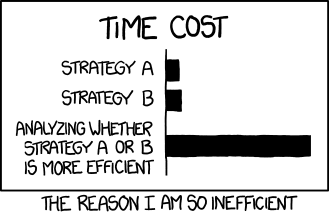
\includegraphics[width=0.5\hsize]{info/xkcd/efficiency.png}
\end{center}

\subsubsection*{Mathe 1}
In Mathe 1 werden euch die Grundlagen der Mathematik beigebracht. Auch hier gibt es Übungsblätter und ein Tutorium in dem diese besprochen werden. Auch hier ist kontinuierliche Mitarbeit sehr zu empfehlen, da die Inhalte direkt aufeinander aufbauen.

\subsubsection*{Einführung in die Kognitionswissenschaft}
Die Einführung in die Kognitionswissenschaft ist eine der beiden Vorlesungen im ersten Semester, in der nur die Kognis sitzen. In dieser Veranstaltung wird euch ein Überblick über die einzelnen Felder der Kognitionswissenschaft gegeben, der fürs weitere Studium sehr nützlich ist.

\subsubsection*{Neurobiologie und Sinnesphysiologie}
In der Veranstaltung Neurobiologie und Sinnesphysiologie werden euch der Aufbau des Gehirns und die einzelnen Verarbeitungsmechanismen näher gebracht. Neben der Vorlesung müsst ihr noch eins von zwei Seminaren wählen, welche sich lediglich in der Uhrzeit unterscheiden. In diesen müsst ihr einen kleinen Vortrag im Themenfeld der Vorlesung halten.

\subsubsection*{Mathematische Statistik I}
In den empirischen Wissenschaften ist das Beherrschen von statistischen Methoden sehr wichtig. In dieser Veranstaltung wird euch der Teil der Statistik näher gebracht, welcher sich mit der Darstellung von empirischen Daten befasst (deskriptive Statistik). 


